\section{Do real compaction mechanisms behave this way?}
\label{sec:experiment}

Everything above describes records chosen \emph{optimally}. No coordinator
chooses a record that way. It keeps a count, or a threshold, or the first few
sub-agents' reports, or hashes the episode into a fixed number of buckets --- and
it does so through a noisy view of what each agent actually did. This section
evaluates those mechanisms, none of which was designed to be optimal, and asks
where they land.

\paragraph{Setup.}
Every profile is enumerated, so the numbers are exact and there is no sampling,
no seed and no error bar. For each mechanism we measure the Bayes reconstruction
error $D$ and the largest all-teammate-profile margin $\gamma$ any bounded
payment rule can extract. The margin is computed \emph{via
Theorem~\ref{thm:elim}}: one LP per agent, rather than a search over payment
rules. The experiment therefore uses the paper's main tool as its instrument.
Under noise, agent~$i$'s effort is observed as $X_i$ with
$\Pr[X_i \ne S_i] = \eta$; the mechanism sees $X$ while reconstruction and
payment are still judged against the true $S$.

Predictions were written down and hashed before the harness was written; two of
them turned out to be wrong, and we report both.

\begin{table}[t]
\centering
\caption{Compaction mechanisms at $n = 5$, uniform prior, no noise. ``Flat''
means $D = \Dnull(K)$ \emph{and} $\gamma > 0$. The last two rows are the same
size and the same distortion.}
\label{tab:mechanisms}
\small
\begin{tabular}{@{}lrrrrl@{}}
\toprule
mechanism & $K$ & $D$ & $\Dnull(K)$ & $\gamma$ & flat \\
\midrule
full        & $32$ & $0.0000$ & $0.0000$ & $1.0000$ & yes \\
count       & $6$  & $1.5625$ & $0.8750$ & $0.2000$ & no \\
threshold   & $2$  & $1.5625$ & $1.5625$ & $0.0000$ & no \\
prefix-4    & $16$ & $0.5000$ & $0.5000$ & $0.0000$ & no \\
prefix-2    & $4$  & $1.5000$ & $1.1250$ & $0.0000$ & no \\
top-2       & $16$ & $0.7188$ & $0.5000$ & $0.0000$ & no \\
hash-10     & $10$ & $1.5000$ & $0.6875$ & $0.0000$ & no \\
\midrule
flat        & $10$ & $0.6875$ & $0.6875$ & $0.5000$ & \textbf{yes} \\
kmedian     & $10$ & $0.6875$ & $0.6875$ & $0.0000$ & no \\
\bottomrule
\end{tabular}
\end{table}

\paragraph{The theory survives contact.}
No mechanism beats the frontier: every one sits on or above $\Dnull(K)$ for its
own $K$, and every two-label mechanism sits on or above the exact frontier of
Theorem~\ref{thm:onebit}. No mechanism below $K = \gtwo(\Qn)$ is flat. These
were derivations rather than guesses --- their failure would have meant a bug or
a false theorem --- but they are checked against records nobody tuned.

\paragraph{The last two rows are the paper.}
At $n = 5$, \texttt{flat} and \texttt{kmedian} use the same ten labels and incur
\emph{the same} distortion $0.6875 = \Dnull(10)$. One admits a payment rule with
margin $1/2$; the other admits none at all, at any price, for any bounded
decoder. Nothing separates them but where the labels were placed. A designer
comparing records on reconstruction quality alone cannot see this difference, and
the same holds at $n = 3$ ($\gamma = 2/3$ against $0$).

\paragraph{Aggregates fail, but not where we predicted.}
We expected \texttt{count} --- ``how many agents succeeded'' --- to have full
margin and poor reconstruction, since one agent's deviation always moves the
count by exactly one. That is what the edge condition
(Corollary~\ref{cor:edge}) suggests. It is wrong. The measured margin is exactly
$1/n$: $0.3333$ at $n=3$, $0.2000$ at $n=5$. The minimax in
Theorem~\ref{thm:elim} is over \emph{mixtures} of teammate profiles, and a
uniform mixture telescopes --- the intermediate shifts cancel and only the two
endpoints survive, leaving $\tfrac{1}{n}$. A point-mass intuition misses this
entirely, which is the clearest illustration we have of why the elimination
theorem is needed rather than its corollary. Aggregates are therefore
\emph{both} margin-poor and reconstruction-poor, and the margin decays with team
size exactly as the label budget argument in Section~\ref{sec:agents} suggests it
should.

\paragraph{A per-agent witness for every agent, or none.}
\texttt{prefix-$m$} retains the first $m$ agents' bits and drops the rest. Its
margin is exactly zero for every $m < n$, at every $n$ tested --- the dropped
agents are invisible, and the margin is a minimum over agents. The design rule is
therefore sharper than ``keep per-agent information'': partial per-agent
retention buys nothing. \texttt{prefix-4} at $n=5$ is the sharpest case, since it
is simultaneously reconstruction-optimal for its budget and worth nothing for
accountability.

\paragraph{Noise, where both our predictions failed.}
We predicted margins would fall continuously with $\eta$. They do not. At
$n = 5$ the margin of \texttt{flat} \emph{rises} from $0.5000$ to $0.5196$ as
$\eta$ goes from $0$ to $0.05$, before falling to $0.4175$ at $\eta = 0.2$. More
strikingly, noise \emph{creates} margin where a deterministic record had none: at
$\eta = 0.1$, \texttt{kmedian} goes from $\gamma = 0$ to $0.1973$ at $n=5$, and
\texttt{threshold} from $0$ to $0.1440$ at $n=3$. The reason is visible once
stated: a deterministic record is insensitive to an agent whose flip does not
change the label, whereas under noise every flip shifts the label
\emph{distribution} a little. Blur can buy accountability.

This does not contradict Section~\ref{sec:threshold}. A record that factors
through the channel is a restricted class of stochastic encoder, so the best it
can achieve is $\Dnull^{\eta}(K) \ge \Dnull(K)$, and we report both baselines
rather than conflating them; no noisy mechanism attains the unrestricted
optimum. The honest reading is that observation noise trades reconstruction for
sensitivity, and that a designer who cannot afford labels may be able to afford
noise instead. We did not anticipate this and do not develop it further here.

\paragraph{The tilted prior, in mechanisms.}
Under a product Bernoulli$(0.7)$ prior the construction built for the uniform
case stops being optimal --- at $n=5$ it incurs $0.7123$ against $\Dnull(10) =
0.3815$ --- and no mechanism at $K = \gtwo(\Qn)$ is flat, as
Corollary~\ref{cor:tilt} requires.


\begin{figure}[t]
\centering
% Generated by make_figures2.py -- do not edit by hand.
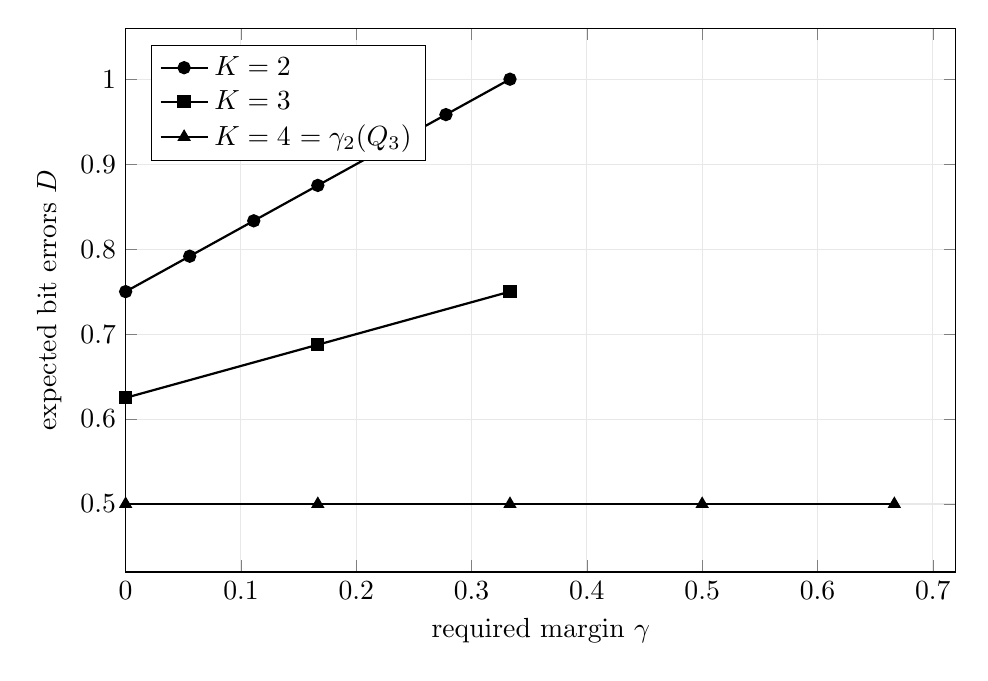
\begin{tikzpicture}
\begin{axis}[
  width=\columnwidth, height=0.70\columnwidth,
  xlabel={required margin $\gamma$},
  ylabel={expected bit errors $D$},
  xmin=0, xmax=0.72, ymin=0.42, ymax=1.06,
  legend pos=north west, legend cell align=left,
  grid=major, grid style={gray!18},
]
\addplot[thick, mark=*] coordinates {(0.000000,0.750000) (0.055556,0.791667) (0.111111,0.833333) (0.166667,0.875000) (0.222222,0.916667) (0.277778,0.958333) (0.333333,1.000000)};
\addlegendentry{$K=2$}
\addplot[thick, mark=square*] coordinates {(0.000000,0.625000) (0.166667,0.687500) (0.333333,0.750000)};
\addlegendentry{$K=3$}
\addplot[thick, mark=triangle*] coordinates {(0.000000,0.500000) (0.166667,0.500000) (0.333333,0.500000) (0.500000,0.500000) (0.666667,0.500000)};
\addlegendentry{$K=4$ $=\gamma_2(Q_3)$}
\end{axis}
\end{tikzpicture}

\caption{The tradeoff at intermediate record sizes, $n = 3$. At $K=2$ it is
the exact frontier of Theorem~\ref{thm:onebit}; at $K=3$ it is shallower and
runs out of feasible margin sooner; at $K = 4 = \gtwo(Q_3)$ it is
\emph{flat}---distortion stays at $\Dnull(4)$ all the way to the maximum
margin $1-1/\dmin = 2/3$. Curves are achievability: each point is a record
that exists. They reproduce $\Dnull(K)$ at $\gamma=0$ and Theorem~\ref{thm:onebit} at $K=2$, both asserted in the harness.}
\label{fig:frontierK}
\end{figure}

\begin{figure}[t]
\centering
% Generated by make_figures2.py -- do not edit by hand.
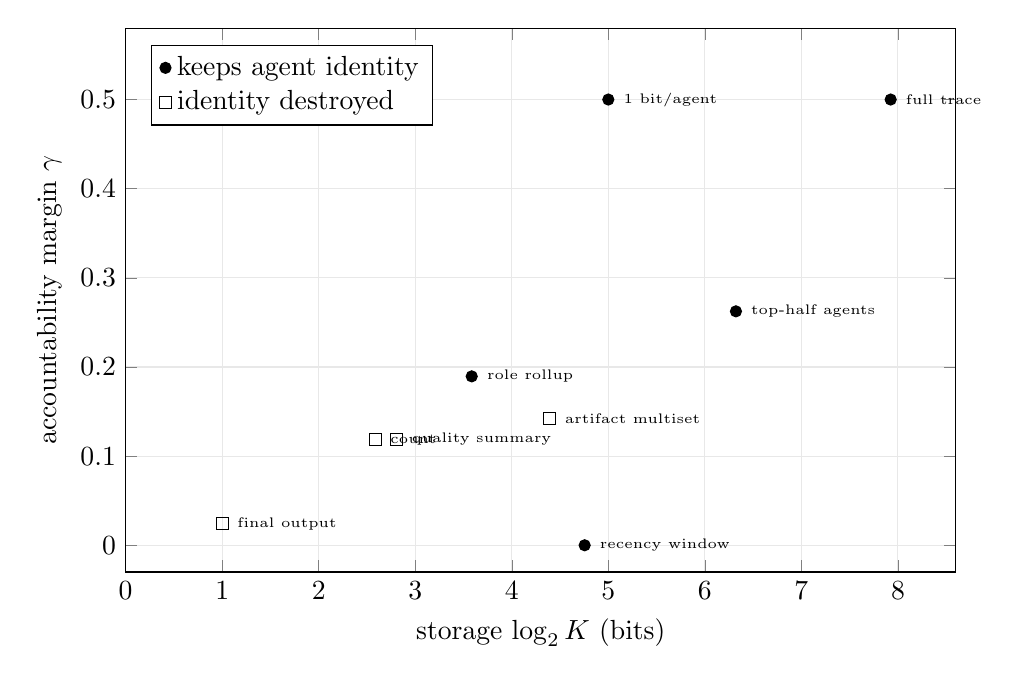
\begin{tikzpicture}
\begin{axis}[
  width=\columnwidth, height=0.70\columnwidth,
  xlabel={storage $\log_2 K$ (bits)},
  ylabel={accountability margin $\gamma$},
  xmin=0, xmax=8.6, ymin=-0.03, ymax=0.58,
  legend pos=north west, legend cell align=left,
  grid=major, grid style={gray!18},
  nodes near coords, point meta=explicit symbolic,
  every node near coord/.append style={font=\tiny, anchor=west, xshift=2pt},
]
\addplot[mark=*, only marks, mark size=2pt] coordinates {(3.5850,0.189474) [role rollup] (4.7549,0.000000) [recency window] (5.0000,0.500000) [1 bit/agent] (6.3219,0.262400) [top-half agents] (7.9248,0.500000) [full trace]};
\addlegendentry{keeps agent identity}
\addplot[mark=square, only marks, mark size=2.2pt] coordinates {(1.0000,0.024300) [final output] (2.5850,0.119020) [count] (2.8074,0.119020) [quality summary] (4.3923,0.142510) [artifact multiset]};
\addlegendentry{identity destroyed}
\end{axis}
\end{tikzpicture}

\caption{Storage against accountability for the episode records at $n=5$.
Records that keep agent identity sit high regardless of how few bits they
use; records that keep content but discard authorship sit low regardless of
how many.}
\label{fig:identity}
\end{figure}
\subsection{An episode, not just a profile}
\label{sec:episodes}

The experiment above compresses the effort profile itself, which concedes the
abstraction most open to question: that what an agent did can be written as one
bit. So we put an episode in between. A coordinator fans out $n$ subtasks; agent
$i$ has a controlled effort bit $S_i$ and returns an artifact whose quality is
drawn from one of two distributions according to it; the coordinator ships iff at
least half the subtasks completed. A \emph{record} now compresses the trace
$(A_1,\dots,A_n,F)$, so the encoder $\enc(\cdot \mid S)$ of
Section~\ref{sec:model} is \emph{measured} rather than defined. Agents are
conditionally independent given $S$, so it is computed exactly by enumerating
artifact tuples. We also ran $200{,}000$ sampled episodes as a cross-check:
they reproduce the exact values to within $0.025$ at $n \le 5$. At $n = 6,7$
the label space outgrows the episode budget --- the full trace alone has $2187$
labels at $n=7$ against $1562$ episodes per profile --- so the empirical
encoder is too sparse there to estimate a margin, and every number we report is
the exact one.

\begin{table}[t]
\centering
\caption{Records over an episode trace, $n = 5$, exact. ``Content'' is not what
buys accountability: \texttt{global\_summary} keeps every artifact and loses only
\emph{who} produced it.}
\label{tab:episodes}
\small
\begin{tabular}{@{}lrrr@{}}
\toprule
record & $K$ & $D$ & $\gamma$ \\
\midrule
full trace              & $243$ & $1.2500$ & $0.5000$ \\
one bit per agent       & $32$  & $1.2500$ & $0.5000$ \\
top-half agents only    & $80$  & $1.2923$ & $0.2624$ \\
multiset of artifacts   & $21$  & $1.9718$ & $0.1425$ \\
count of completions    & $6$   & $2.0194$ & $0.1190$ \\
final output only       & $2$   & $2.1118$ & $0.0243$ \\
\bottomrule
\end{tabular}
\end{table}

\paragraph{Identity, not volume.}
The ordering of records by margin follows how much \emph{per-agent identity}
survives, not how many bits do. We pre-registered this as a quantitative
claim---that removing identity costs proportionally more margin than it saves
storage---and it holds in every matched-storage comparison at every
$n \in \{3,\dots,7\}$: the ratio of relative margin lost to relative storage
saved never drops below $1.07$, with a median around $1.4$--$2.3$. We also
predicted that ratio would exceed $3$ everywhere and that it would grow with
$n$; both were wrong. The direction is robust and the magnitude is usually
modest, with the striking cases being specific pairs rather than the rule. \texttt{multiset of artifacts} retains every
artifact in full and discards only the association between artifact and author;
it keeps far more of the trace than a single bit per agent, and has less than a
third of the margin. At $n = 3$ it even has \emph{more} labels ($10$ against
$8$) and still less than half the margin. This is the design rule stated as a
measurement: accountability is priced in attribution, not in volume.

\paragraph{One bit per agent is not a compromise.}
At both $n$ tested, \texttt{one bit per agent} matches the \emph{full trace} on
both axes exactly---$D = 1.2500$ and $\gamma = 0.5000$ at $n = 5$, using $32$
labels against $243$. We did not predict this. Under this episode model the
per-agent bit is a sufficient statistic for both jobs, so the $7.6\times$
compression is free in the strong sense: nothing about reconstruction or
accountability is given up.

\paragraph{Where we were wrong again, and what it teaches.}
We predicted that retaining bits for only the top half of agents would give
margin exactly $0$, as fixed truncation does in Table~\ref{tab:mechanisms}. It
does not: it keeps $0.2624$ of the available $0.5000$. The difference is that
\emph{which} agents are retained is itself determined by what they did, so an
agent who shirks changes its own probability of appearing in the record. Selection
that depends on behaviour is far better than selection fixed in advance, which
sharpens the rule from Section~\ref{sec:agents}: a record may drop agents, but not
on a schedule decided before the episode. We also predicted the coordinator's
ship/no-ship bit would be worth nothing; it retains a small margin that decays
quickly in $n$ ($0.0900$ at $n=3$, $0.0243$ at $n=5$).
